\documentclass[12pt]{article}
\usepackage{amsmath}
\usepackage{amssymb}
\usepackage{geometry}
\usepackage{enumerate}
\usepackage{natbib}
\usepackage{float}%稳定图片位置
\usepackage{graphicx}%画图
\usepackage[english]{babel}
\usepackage{a4wide}
\usepackage{indentfirst}%缩进
\usepackage{enumerate}%加序号
\usepackage{multirow}%合并行
\title{\large UM-SJTU JOINT INSTITUTE\\Advanced Lasers and Optics Laboratory\\(VE438)\\\ \\\ \\\ \\\ \\\ \\\ \\\ \\\ \\\ \\\ \\\
Post Lab Assignment\\\ \\\ LAB 4\\\ Optical Communication \\\ \\\ \\\ \\\ \\\ }
\author{Name: Pan Chongdan \\ID: 516370910121}
\date{Date: \today}

\begin{document}
\maketitle
\newpage

\section{Experiment Result}
\begin{figure}[H]
\centering
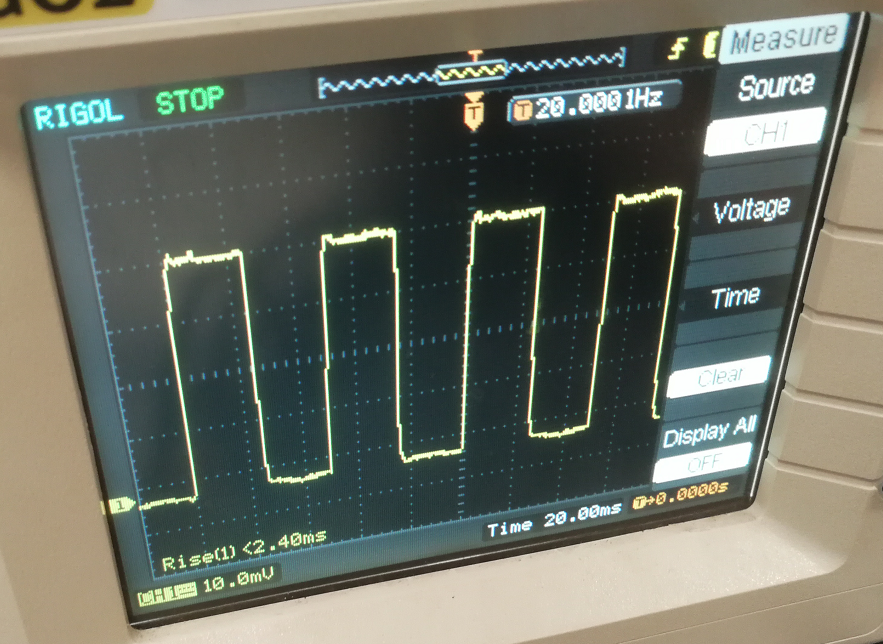
\includegraphics[scale=0.4]{Q2P1.png}
\end{figure}
\begin{figure}[H]
\centering
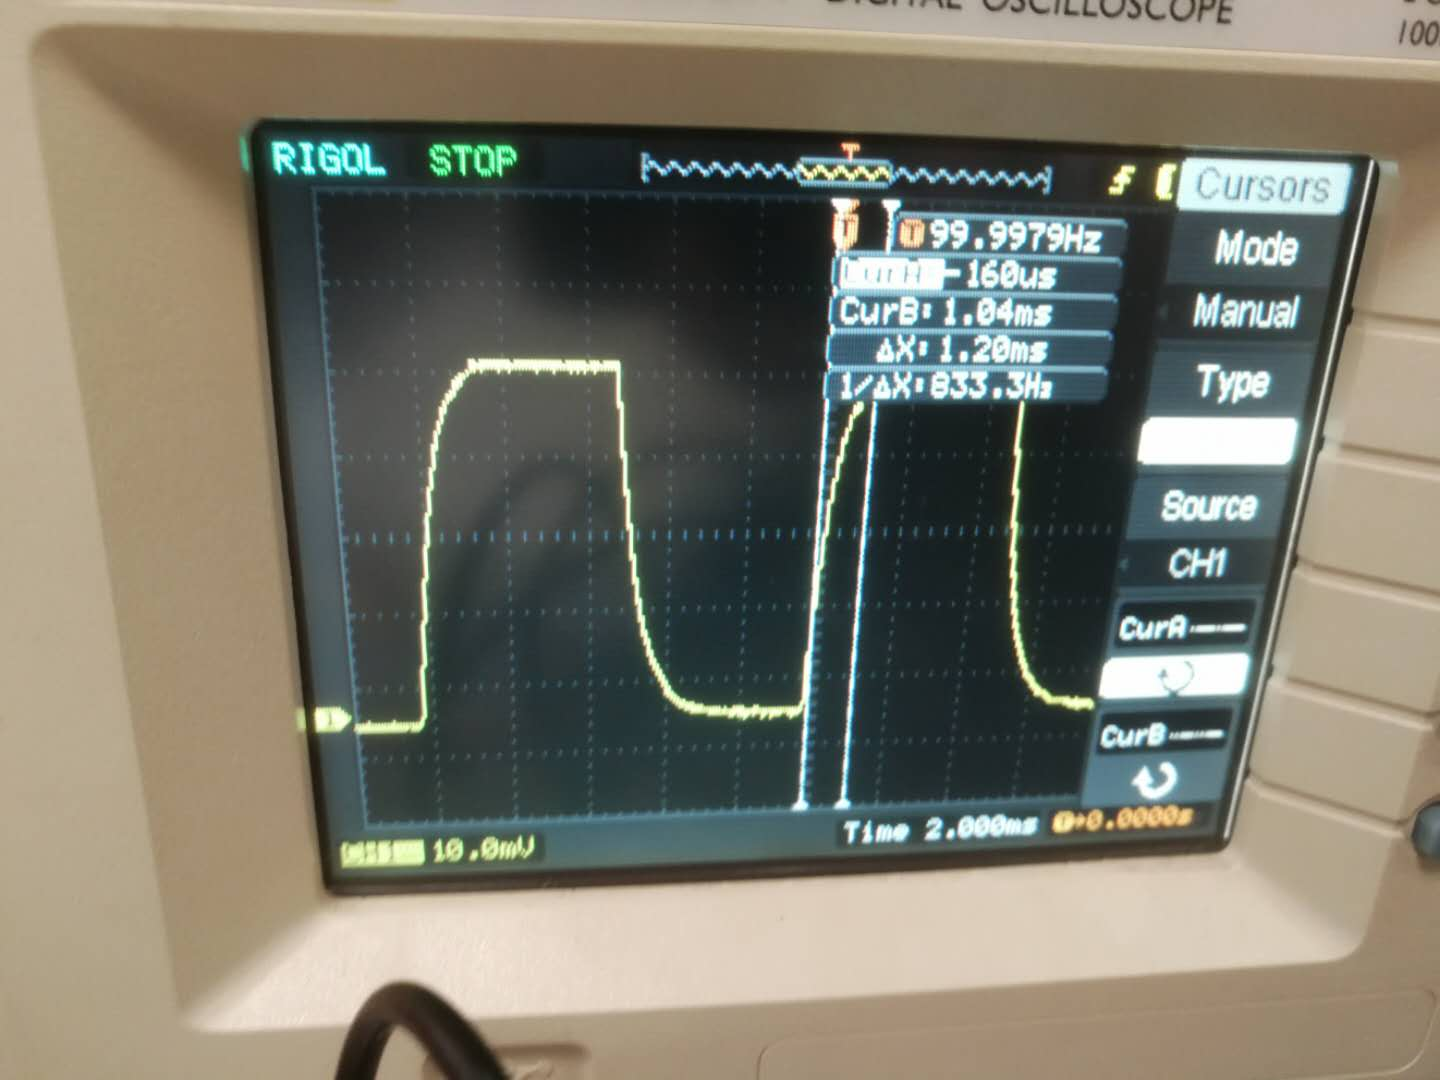
\includegraphics[scale=0.2]{Q2P2.jpg}
\end{figure}
\begin{figure}[H]
\centering
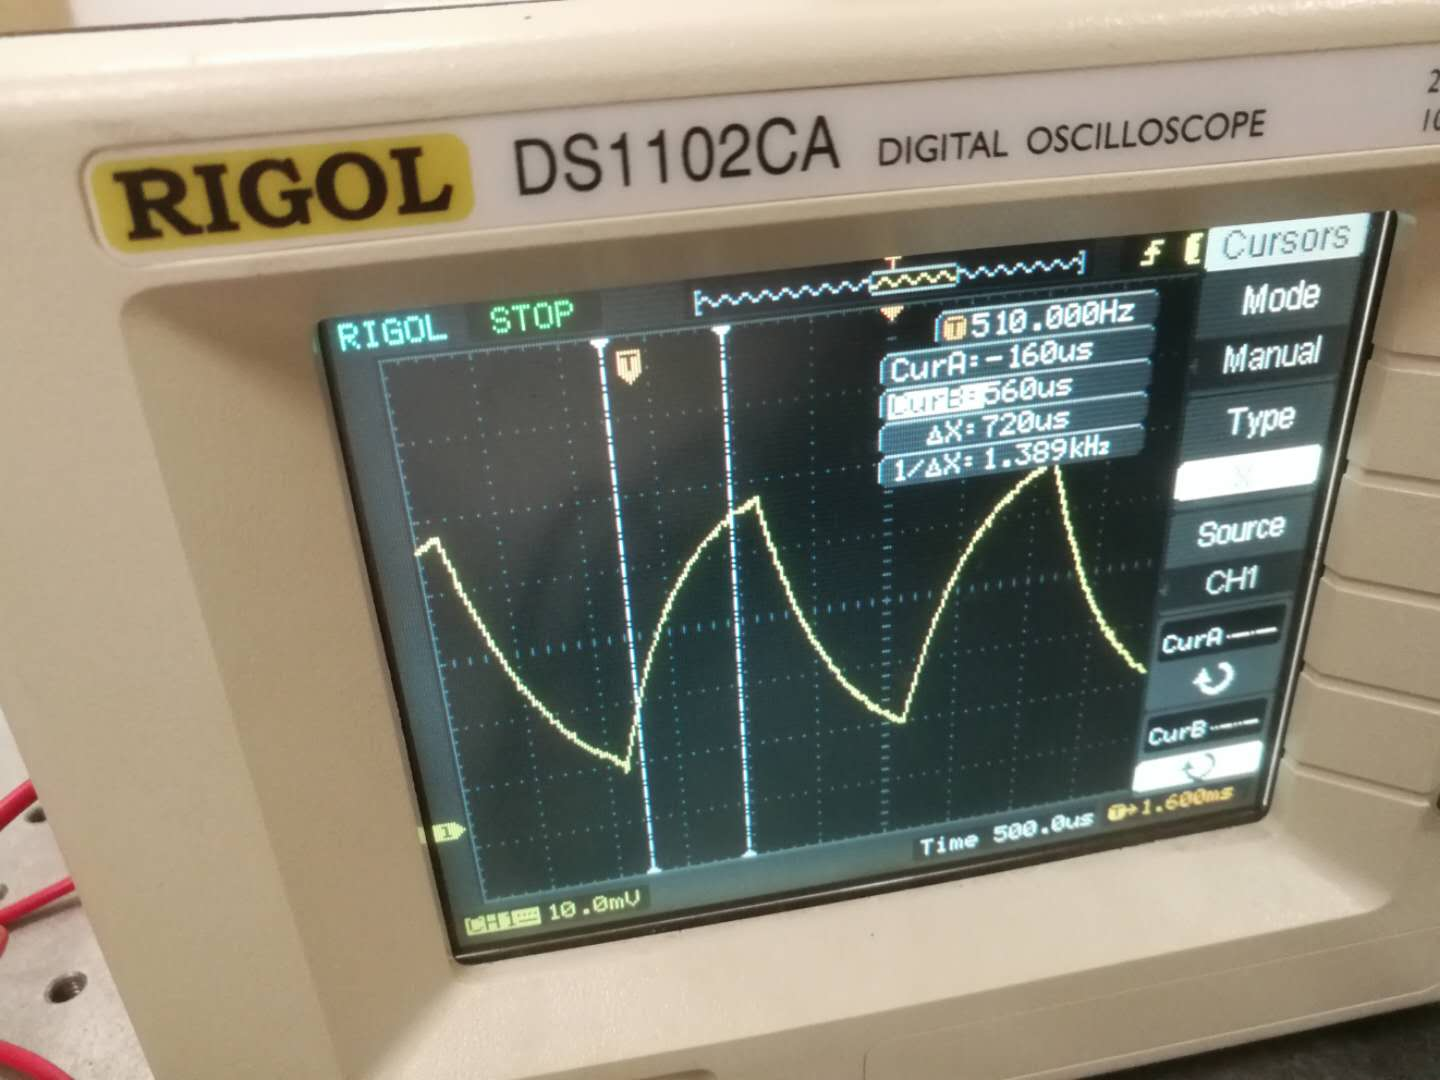
\includegraphics[scale=0.2]{Q2P3.jpg}
\end{figure}
When the frequency is 20 Hz, the rise time is about 2.4 ms, when the frequency is 100 Hz and 500 Hz, the rise time becomes 1.2 ms and 720 us. So the rise time decreases as the the frequency increases. Also, it's worth to mention that the rise time for 500 Hz is not exactly the actual rise time, because the wave haven't reach 90\% of its maximum value. 
\begin{figure}[H]
\centering
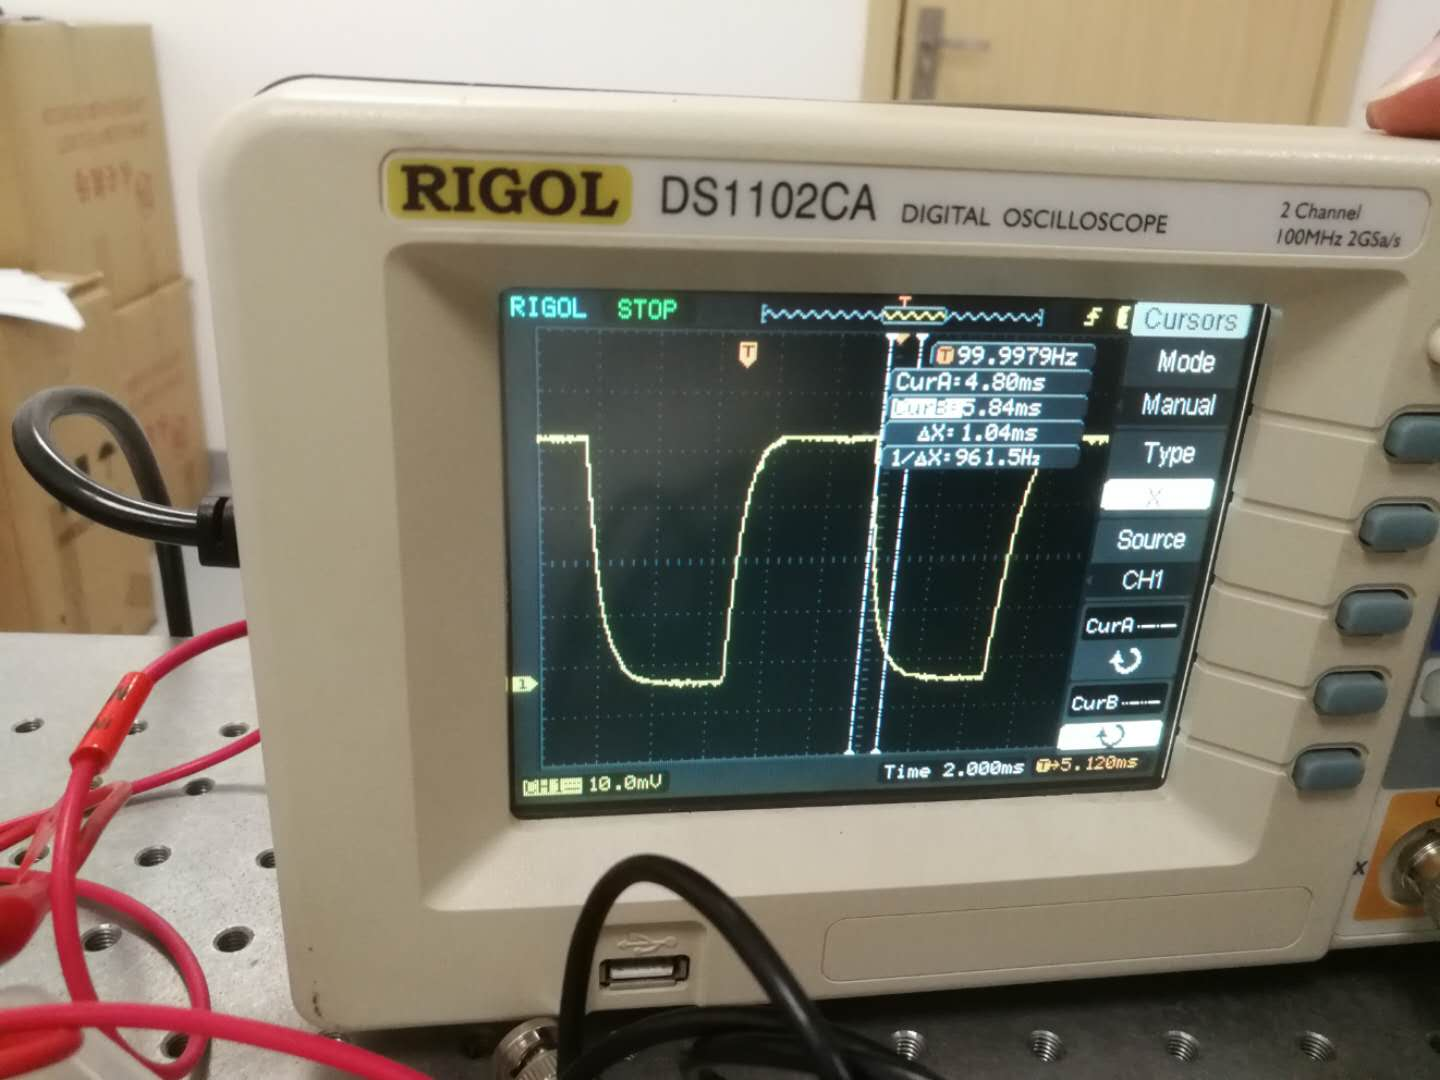
\includegraphics[scale=0.2]{Q2P4.jpg}
\end{figure}
\begin{figure}[H]
\centering
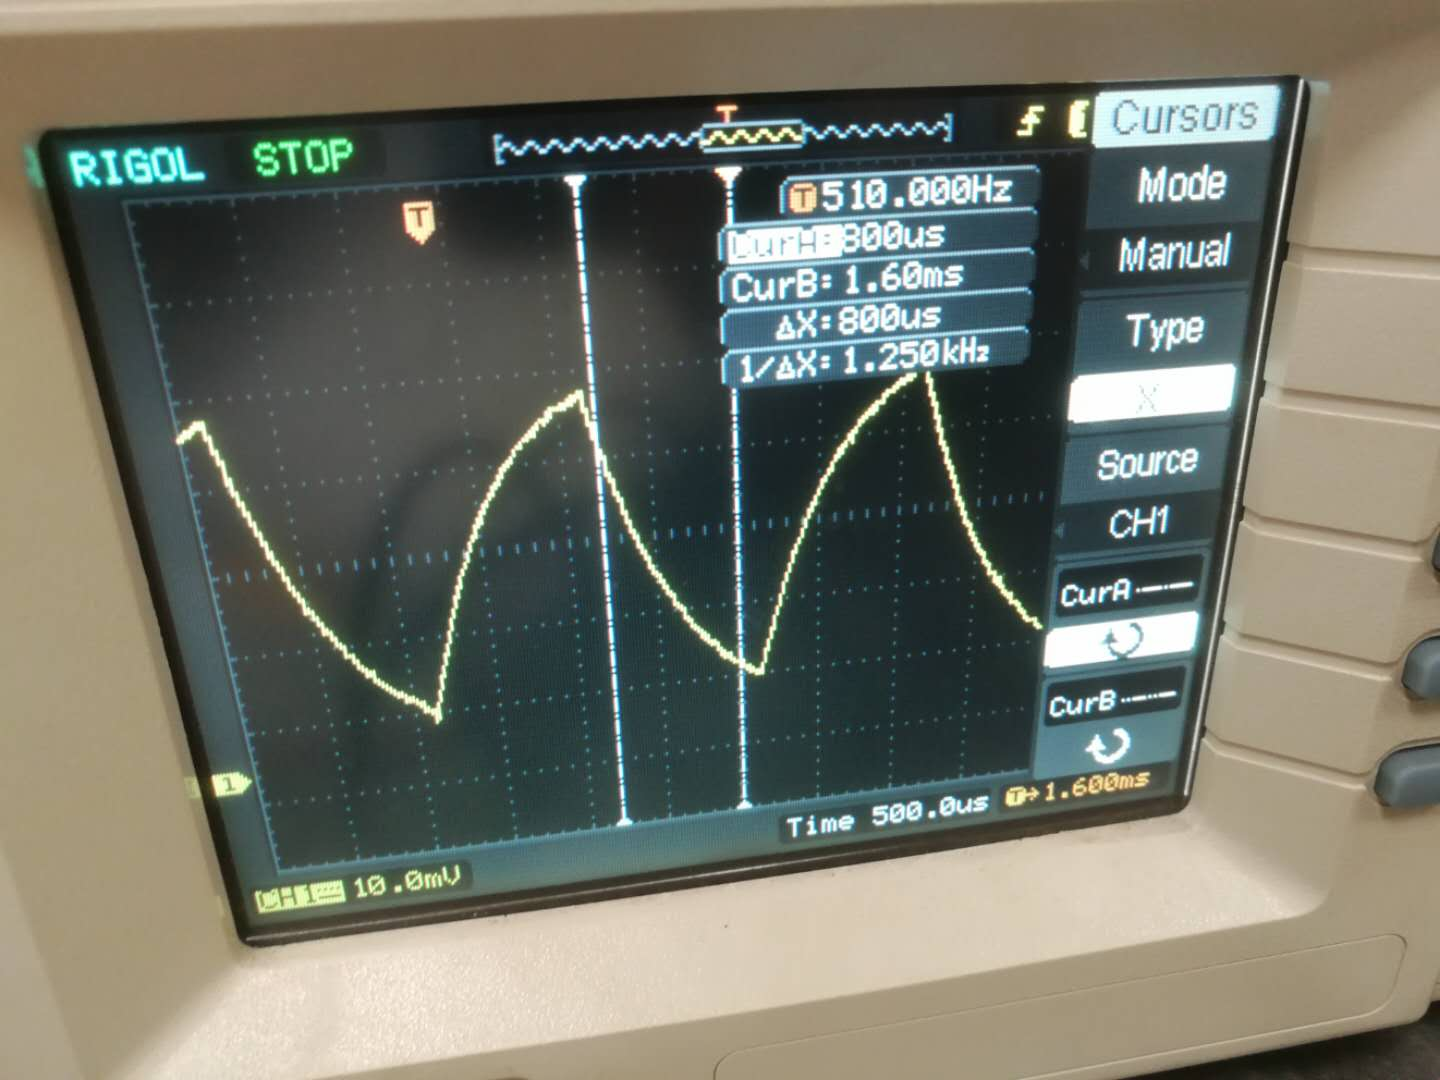
\includegraphics[scale=0.2]{Q2P5.jpg}
\end{figure}
The fall time is similarly for rise time, which decrease as frequency increase. And 800 us doesn't fully represents for the actual fall time.
\begin{figure}[H]
\centering
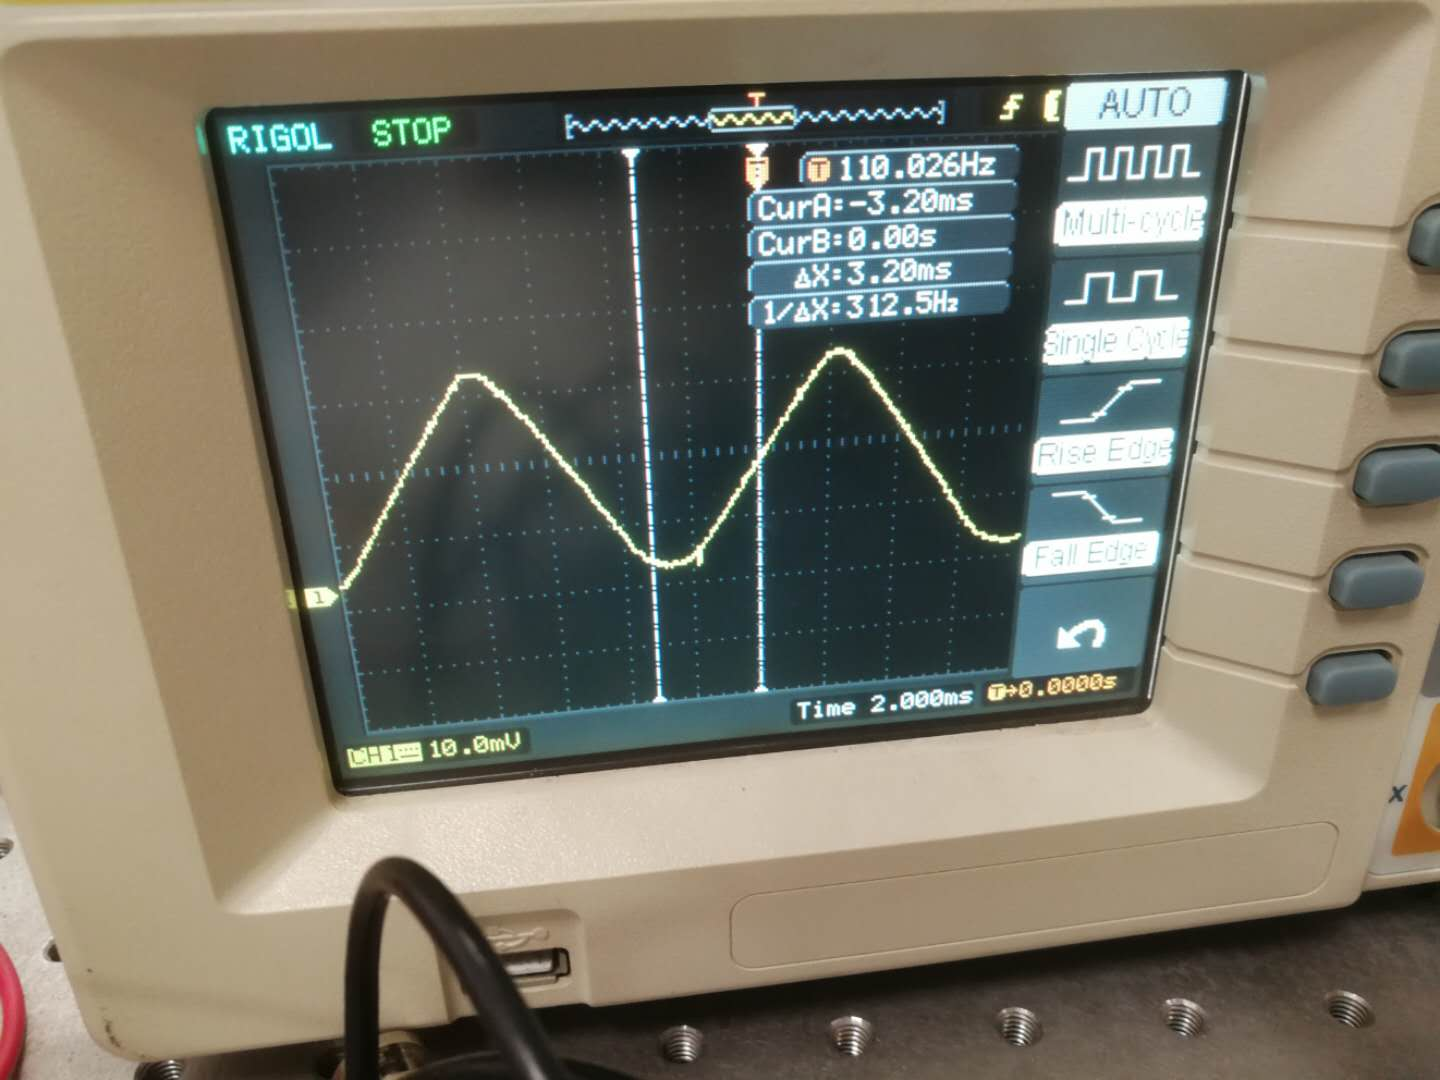
\includegraphics[scale=0.2]{Q2P6.jpg}
\end{figure}
When we set the higher bias around 3.5 V and lower bias around 3.08 V. As we increase the higher bias voltage, the voltage difference for the laser diode becomes lower, and it's harder for us to observe the triangle pattern, especially for the peaks because the intensity of the light also decreased.
\section{Answers for Post Lab Questions}
\subsection{Question 1}
For the transmit end, we must set an interval large enough between high level signal and low level signal so that the semiconductor laser diode can emit light of enough intensity, otherwise it's hard for the receive end to distinguish the signal. However, the input voltage signal can't be too big because it may break the diode. In addition, we must first regulate the emitting device so that the light emitted is horizontal and can shoot to the receive end accurately. Another limitation for the transmit end is the frequency which can't be to high because it'll hard for the diode to generate the signal.
\par For the receive end, the laser light should be focused into the multi-mode fiber with high accuracy in a very close distance so that the signal can be generated. I think the transmitting efficiency is a limitation for the receive end because it's very hard for single-mode fiber to generate a signal that can be detected by the oscilloscope
\subsection{Question 2}
According to the photos in experiment results, when the input is a square wave and the frequency is 20Hz, we observed the signal in a shape of square wave. As the frequency increases, the peak becomes closer and closer and when the frequency is 500 Hz the signal is no longer like a square wave. Finally, the signal is very similar to triangle wave when the frequency is higher. I think it's because there is a rise time and fall time for the diode and the signal started to fall before it reached its maximum value. As a result, the frequency can't be set to high.
\subsection{Question 3}
We can apply the wave length division multiplexing technology by putting a multiplexer and demultiplexer at the transmit end and receive end respectively. In this case, the receiver can refit the receive end so that it can have two focus and the light can be focused on two different photon diodes, since they have different focal length so that they can only detect one color. Then we can distinguish the different signals. Another way is use two photon diodes of different and narrow bandwith so that they can't be disturbed by light of other color but it still can get the signal.
\end{document}